\section{Result 4}

\subsection*{The MapReduce function}
todo

\subsection*{The List function}
todo


\subsection{Correlation analysis}
As shown in \ref{run3-chart1}, there is a correlation between a students achieved grade and the amount of time they spend on Sakai, although the correlation isn't particularly strong. \ref{run3-chart2} shows that relative change in class ranking is not related to Sakai usage for the CSC1015F course.


\begin{figure}[H]
    \centering
    \begin{mdframed}
        \centering
        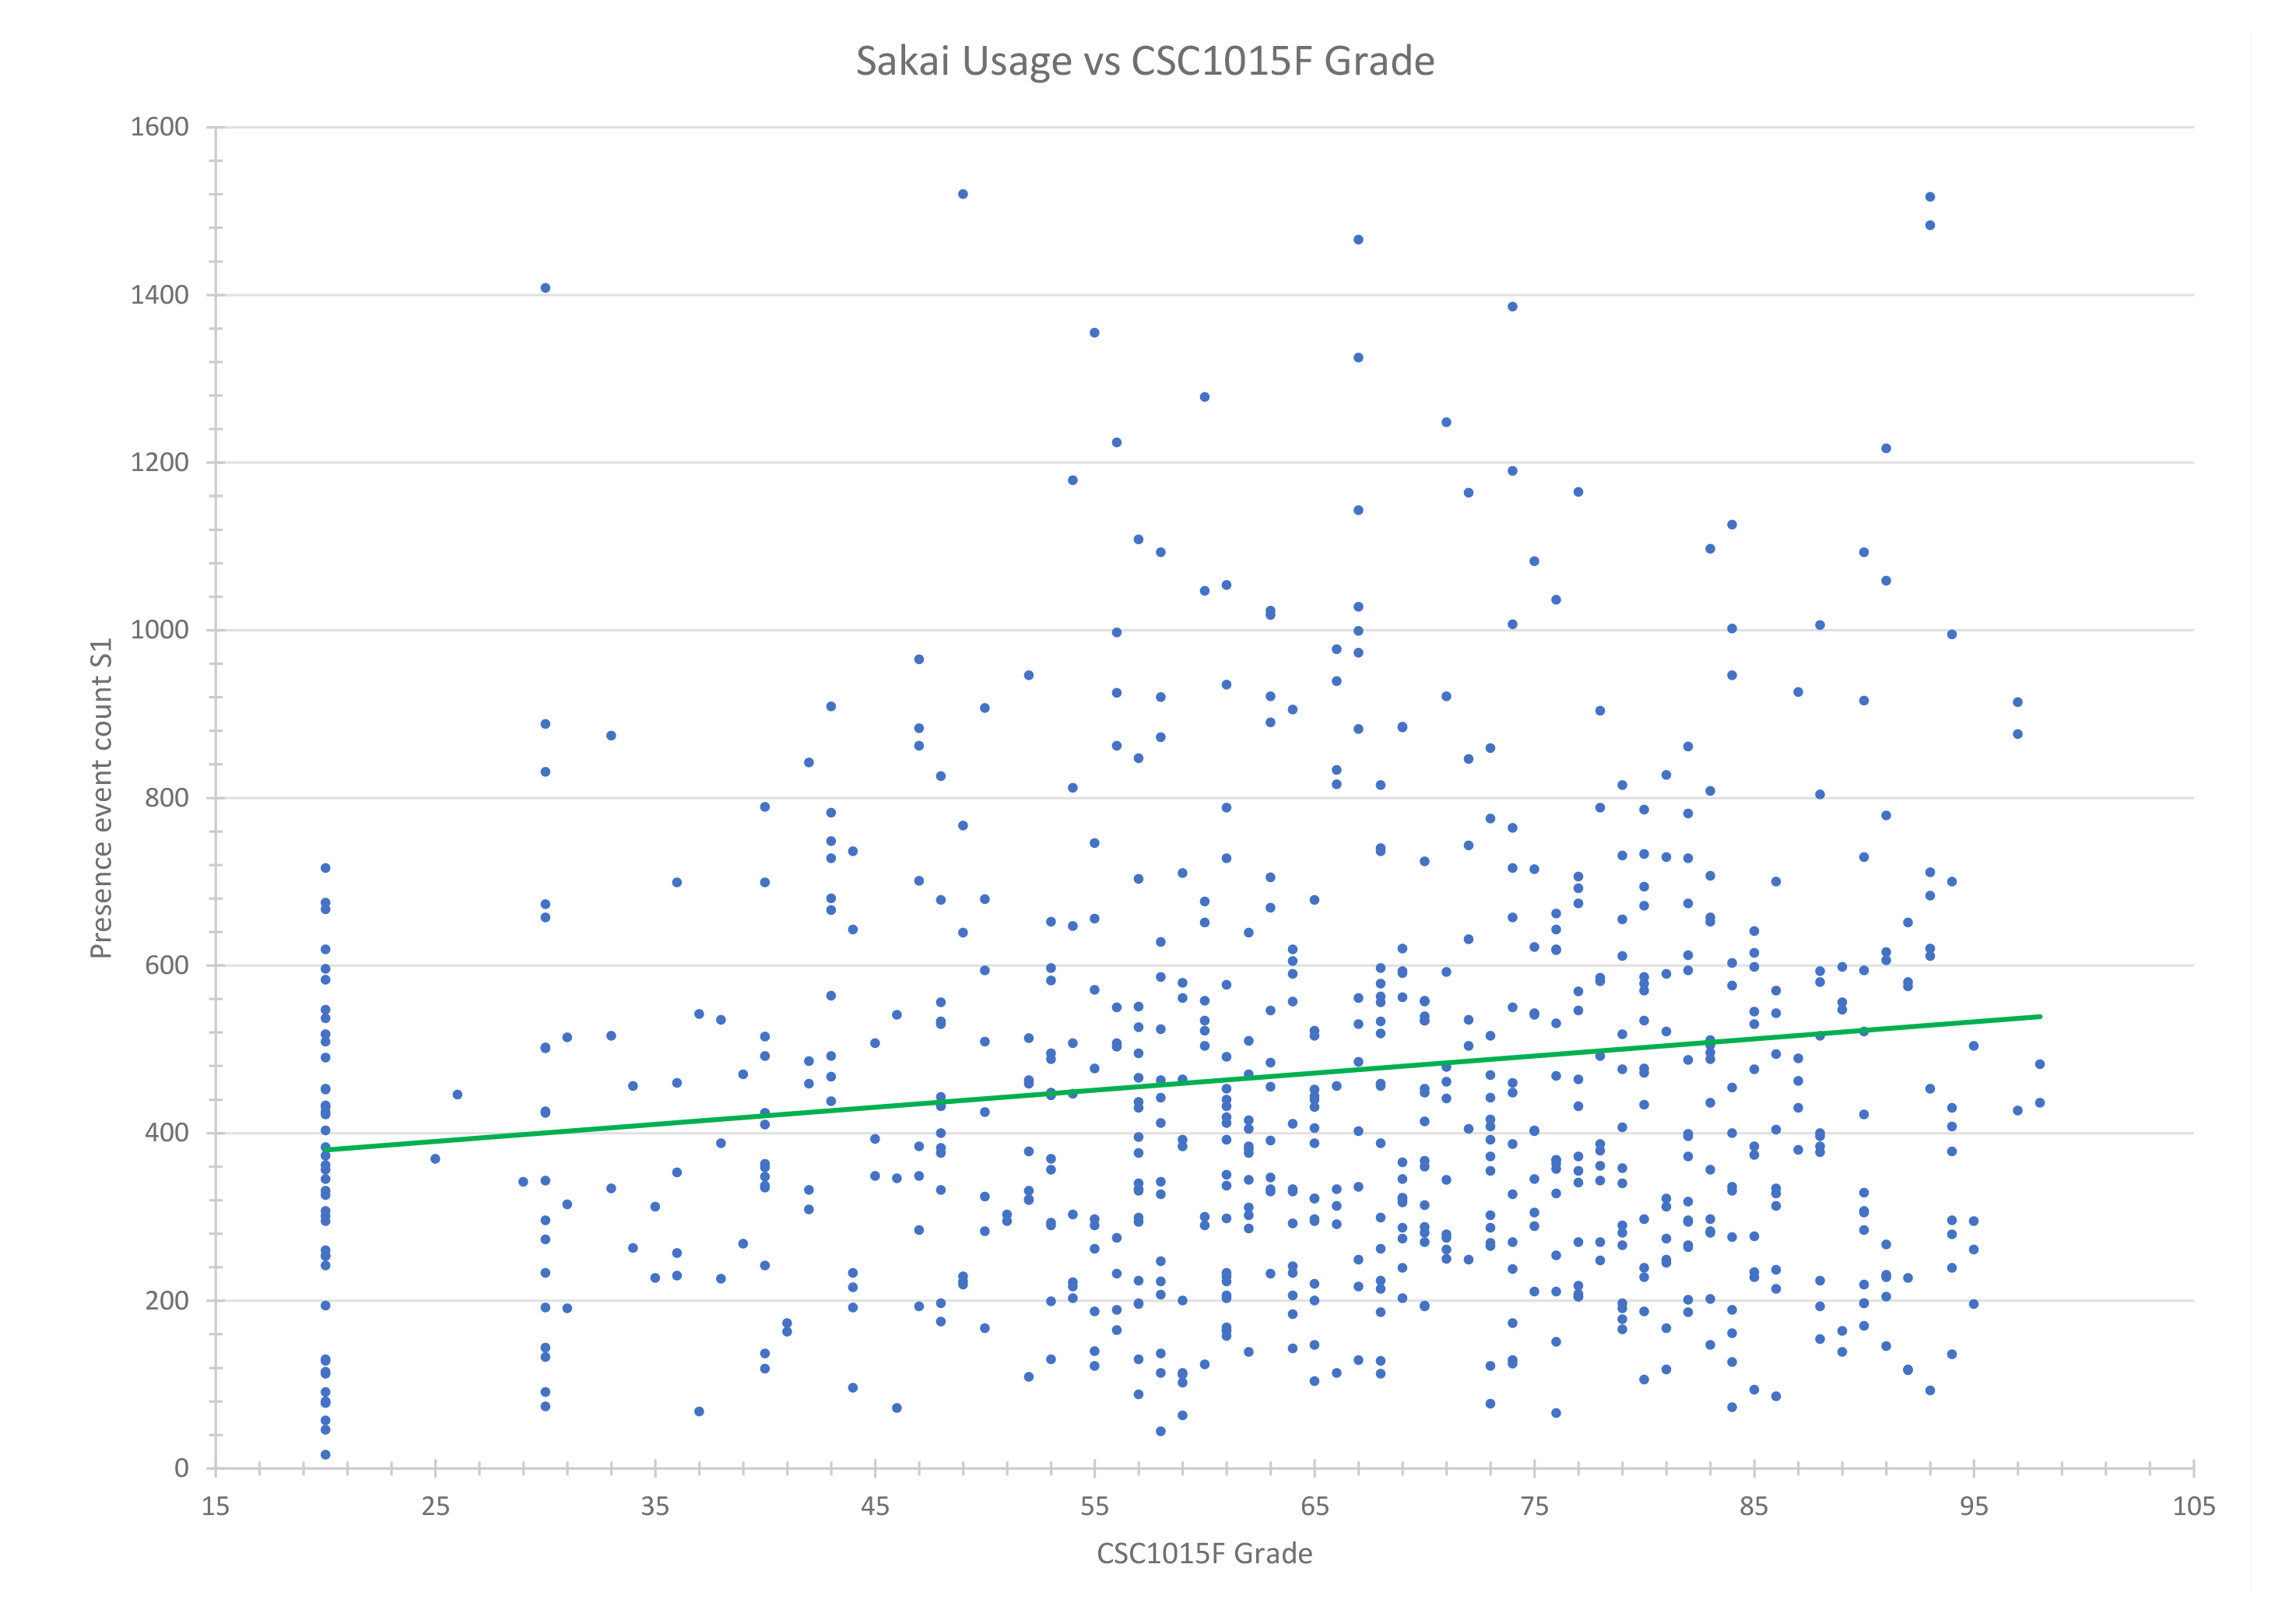
\includegraphics[scale=0.55]{./resources/figures/run3-chart1.png}
    \end{mdframed}
    \caption[CSC1015 grade vs general Sakai usage]{\textbf{Figure \ref{run3-chart1}: Correlation between students' general Sakai usage and CSC1015F results.} The count of a student's presence events on the Sakai platform seems to show a slight correlation with grade achieved in the CSC1015F course.}
    \label{run3-chart1}
\end{figure}

\begin{figure}[H]
    \centering
    \begin{mdframed}
        \centering
        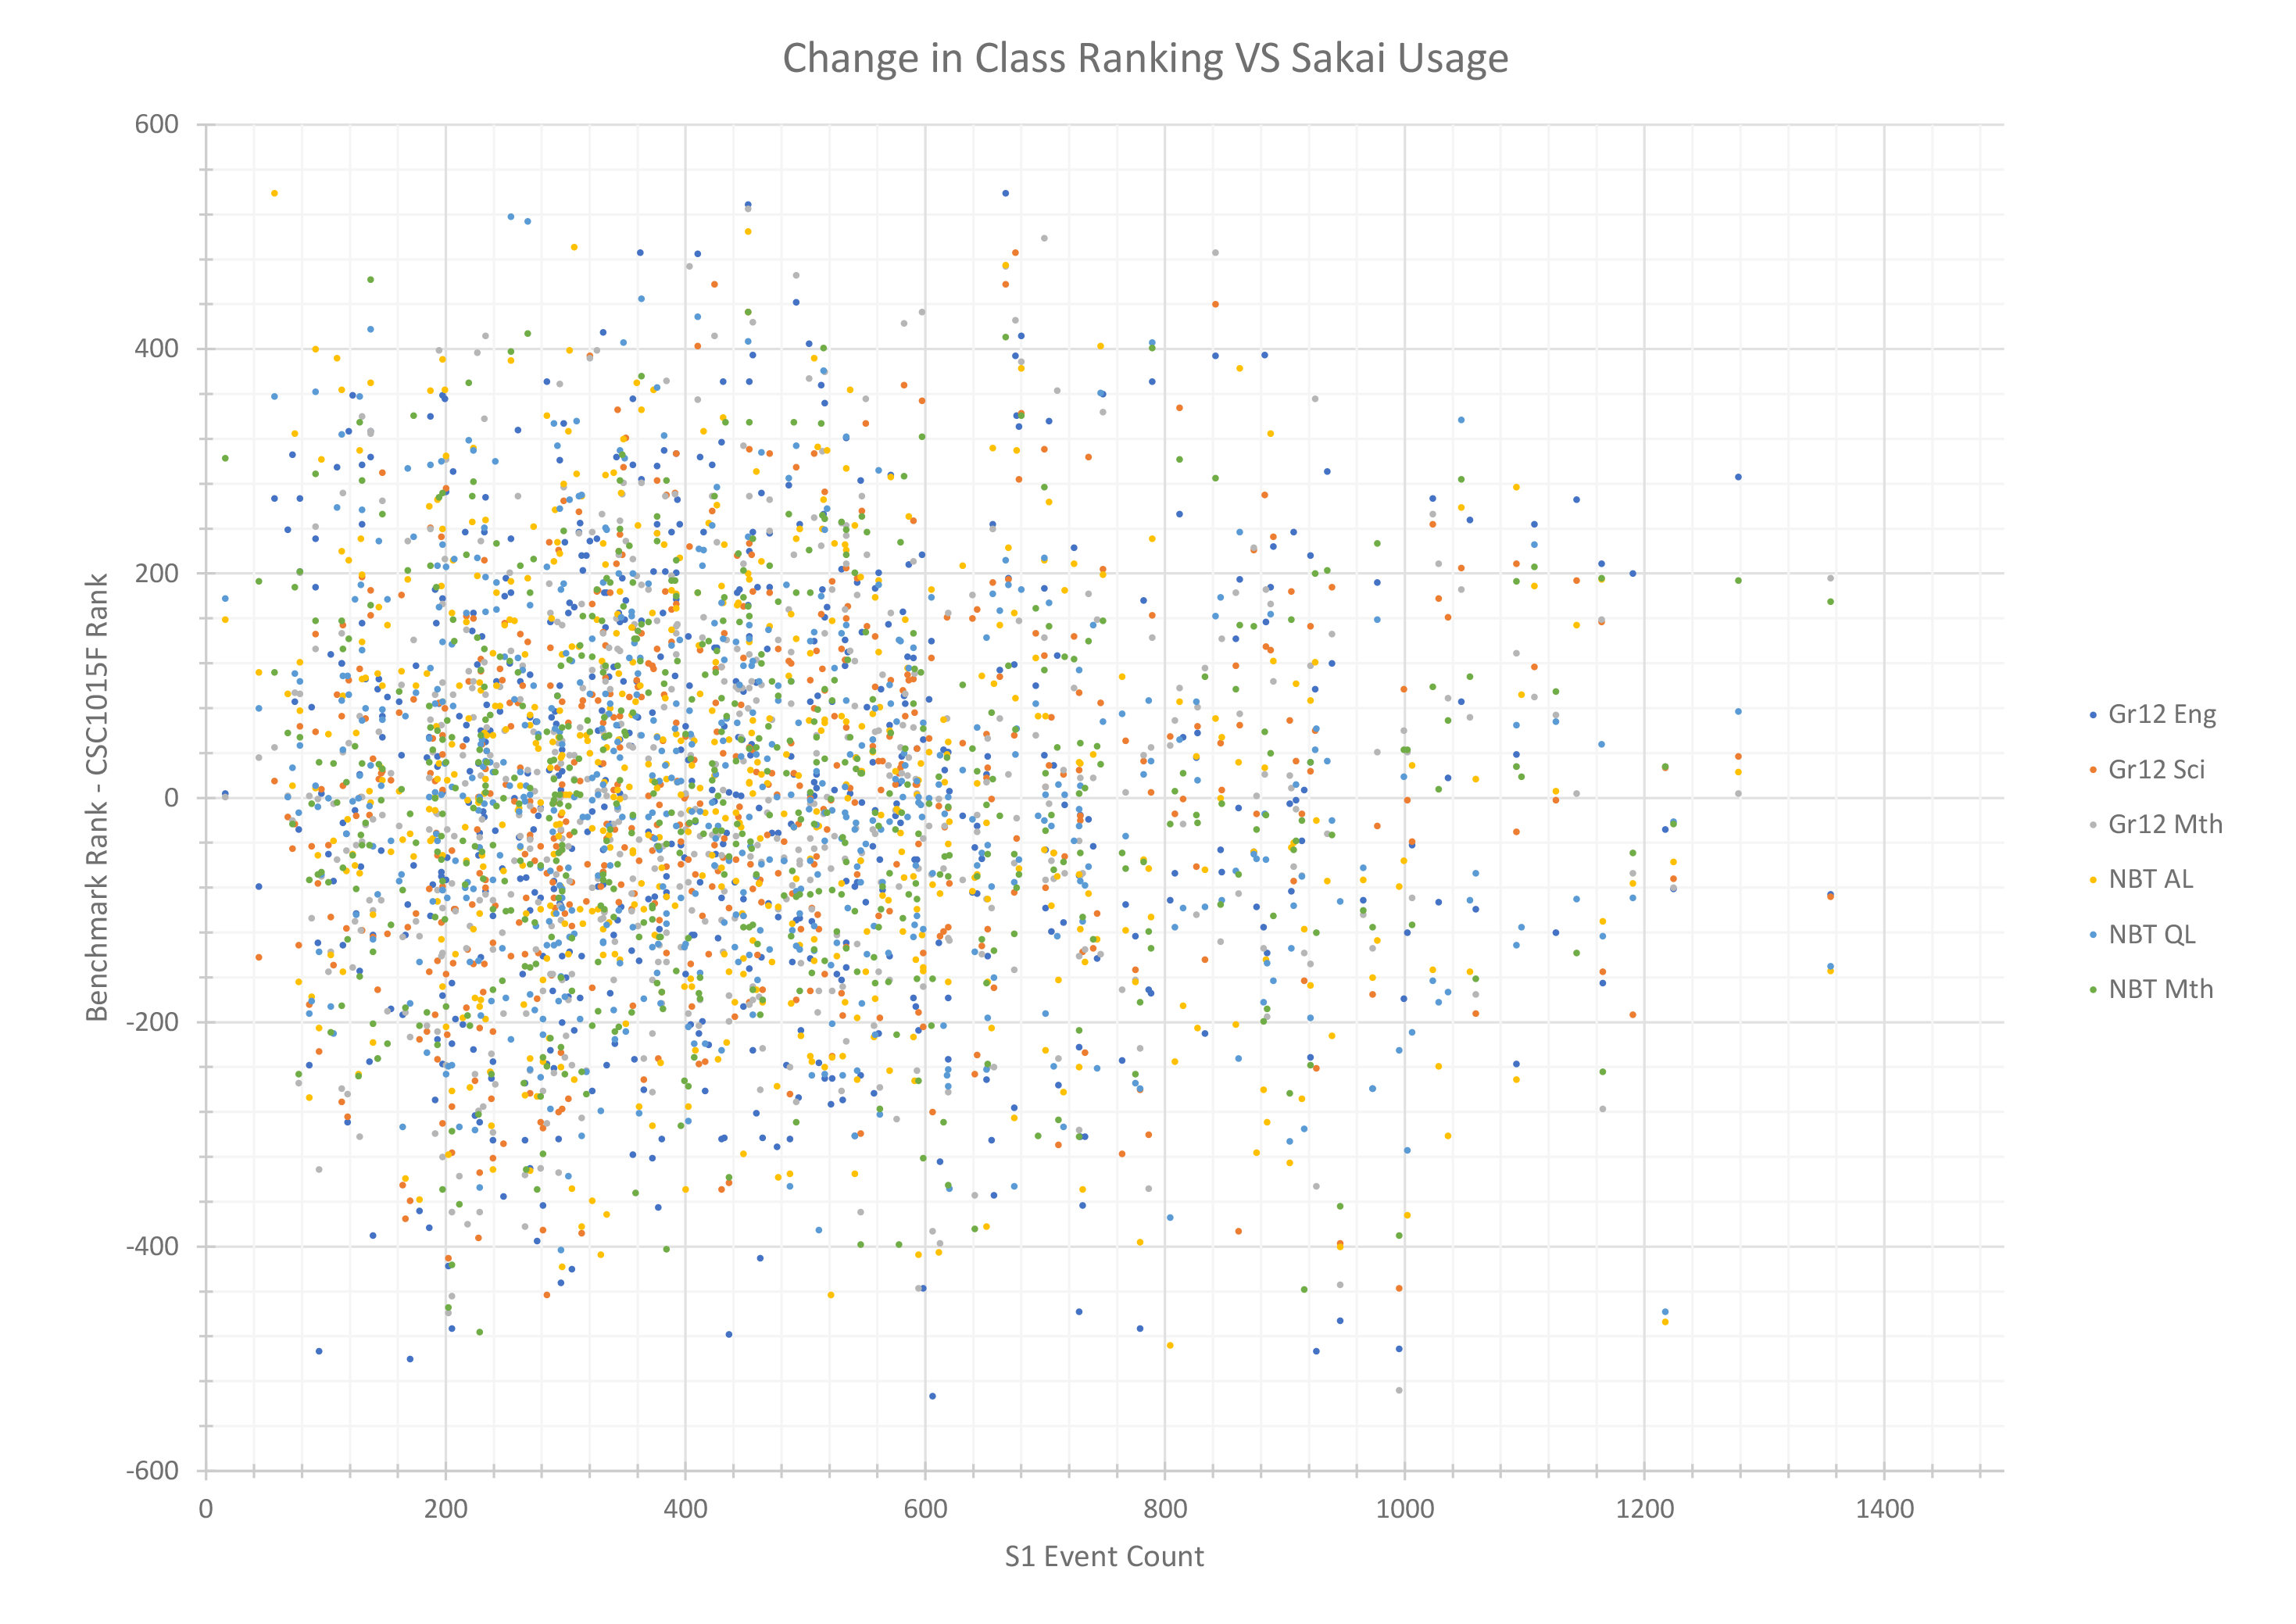
\includegraphics[scale=0.55]{./resources/figures/run3-chart2.png}
    \end{mdframed}
    \caption[Change in class ranking vs Sakai usage]{\textbf{Figure \ref{run3-chart2}: Change in class ranking vs Sakai usage.} This chart shows the number of times a student logs into the Sakai platform compared to the change in their class ranking from benchmark tests to course result. To achieve this dataset, a student's ranking (R) is calculated for the final CSC1015F grade, and separately for each benchmarking test (shown in the key). The change in ranking is worked out as $CSC1015F R - Benchmark R $, with a positive R indicating that the student improved relative to their peers. This graph doesn't show a strong correlation between R and Sakai Usage}
    \label{run3-chart2}
\end{figure}